\chapter{Operation}
The user operation of Impetus can be divided into two parts: the
actual usage of the alarm component, and scheduling and other Twitter
features.

\section{Alarm}
One of the more important steps in operating this device is making
sure that the temperature sensor is has line of sight of where the
user's head will be in bed. While in the ideal case, the temperature
sensor would sense human presence on any part of the body, clothing
often affects the body's luminosity, leading to temperature readings
very close to the ambient threshold. The head not only avoids this
problem (except that hair affects luminosity as well), but also
benefits by being the part of the body that outputs the most heat. The
alarm should also be placed so that the user cannot be further than 5
feet away from the temperature sensor for reasons discussed earlier.

The Raspberry Pi within the device needs to be connected to a 5V power
source via a micro USB cable. An Ethernet cable is optional if the
device already has an alarm configuration and the user doesn't want to
use any impromptu alarms. When the Raspberry Pi is powered up, the
Arduino Pro Mini also begins (it is powered by the Raspberry Pi), and
the Impetus program on the Raspberry Pi will begin on start up.

The alarm consists of three different states with different user
requirements: the idle state, the sleep state, and the alarm state.

\subsection{Idle State}
In the idle state, the temperature sensor constantly reads in an
attempt to find a temperature above the ambient threshold. If it finds
a temperature above that, it will transition to the sleep state if it
stays above the threshold for a minute. Therefore, if the user wishes
to go to sleep, they must be in front of the sensor for a minute to
activate it. If they do not wish to enter that state, they must not be
in front of the device for more than a minute at a time. It is
important to the position Impetus in a way that avoids that from
happening.

\subsection{Sleep State}
Being in the sleep state can be determined by checking if the
right-most dot on the display is lit and the display is half as
bright. In this state, the user doesn't have to do anything to
transition to the alarm state -- that transition is dependent on the
alarm time the Raspberry Pi sets as the device transitions into the
sleep state. To repeat: The alarm time is set as the user transition
the device into the sleep state. That time will not change, though the
device will accept new alarm schedules while in this -- or any --
state. In a similar vein, it is important to note that alarms will
never go off unless the user transitions to the sleep state. When the
alarm time is met, the device transitions to the alarm state.

In the sleep state, the device sensors measure temperature and volume
over the course of sleep. The nature of temperature readings from this
sensor in conjunction with volume readings allows the user to
extrapolate data like movement in sleep.

\subsection{Alarm State}
The alarm state is characterized by all digit dots being lit, as well
as a buzzer turning on and off on a one-second interval (though the
buzzer may silence itself before the transition to a new state). In
order for the user to transition away from the alarm state, they must
move away from the temperature sensor for 60 consecutive
seconds. After the initial 10 seconds, the buzzer should stop its
intermittent buzzing. If the user becomes detected by the device
between 10 and 60 seconds, however, the buzzer will begin again, and
the count will be reset. If the user never leaves the field of view of
the temperature sensor, the device will never leave the alarm state.

\section{Twitter}
Twitter serves two purposes for Impetus: it is the service used to
receive scheduling messages, and it is the service used to send
statistics to the user. To make use of these (and these are required),
the user must create a Twitter alias and application for the
device. The user should then have the necessary tokens and secrets for
the configuration file found on the Raspberry Pi.

\subsection{Alarm Scheduling}
To either schedule an alarm or unschedule an alarm, you must send a
direct message to the device's Twitter alias. There are two base
commands you can send the device: \verb|set| and \verb|stop|.

\verb|set| can either take one argument for an ``impromptu'' alarm, or
two arguments for a weekly alarm. In both cases, the right-most
argument should be in the form \verb|HH:MM|, where \verb|HH|
represents an hour between 00 and 23, and \verb|MM| represent a minute
between 00 and 59. The argument must always have 5 characters in
total. If you are scheduling a weekly alarm, the first argument is the
full name of the weekday for which you are scheduling. \verb|set|
overwrites existing values, so caution is advised.

Be wary of ``impromptu'' alarms: if one is set and the time is later
in the day, Impetus will choose it and remove it from the
scheduler. But if it's set but would come earlier in the day, then
Impetus prefers to set the next alarm to the current day's alarm. If
it cannot set it to that, then the device will set the alarm to the
next day at the impromptu time without regard to the next day's alarm
time. Furthermore, Impetus will have unexpected behavior if you
attempt to transition into the sleep state when the next available
alarm is not for tomorrow.

\verb|stop| either takes no arguments or one argument (a full name of
a weekday). With no arguments, \verb|stop| erases the impromptu alarm
if it is set. With one argument, \verb|stop| erases the alarm for the
weekday for which the argument was chosen.

If a \verb|set| or \verb|stop| completes successfully, you will
receive a direct message back from the device declaring that.

\begin{figure}[h!]
  \centering
  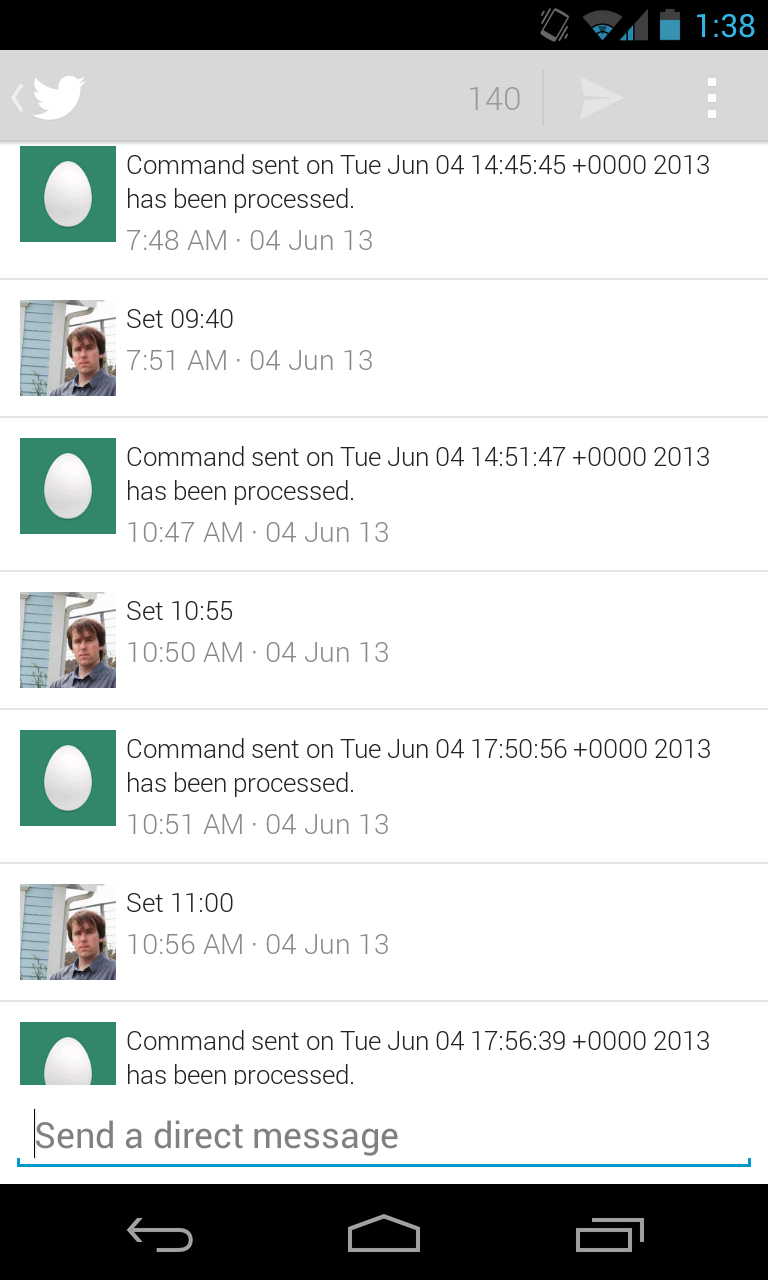
\includegraphics[width=0.5\textwidth]{twitop}
  \caption{A couple \texttt{set} commands with acknowledgement.}
\end{figure}

\subsection{Retrieving Metrics}
Statistics are generated during the transition between the sleep and
alarm states. They are then sent to the timeline of the device's
Twitter alias, which should be marked as protected. These statistics
are images of graphs, so if the user has the correct permissions to
see the device's tweets, the user will be able to see the statistics.

\begin{figure}[h!]
  \centering
  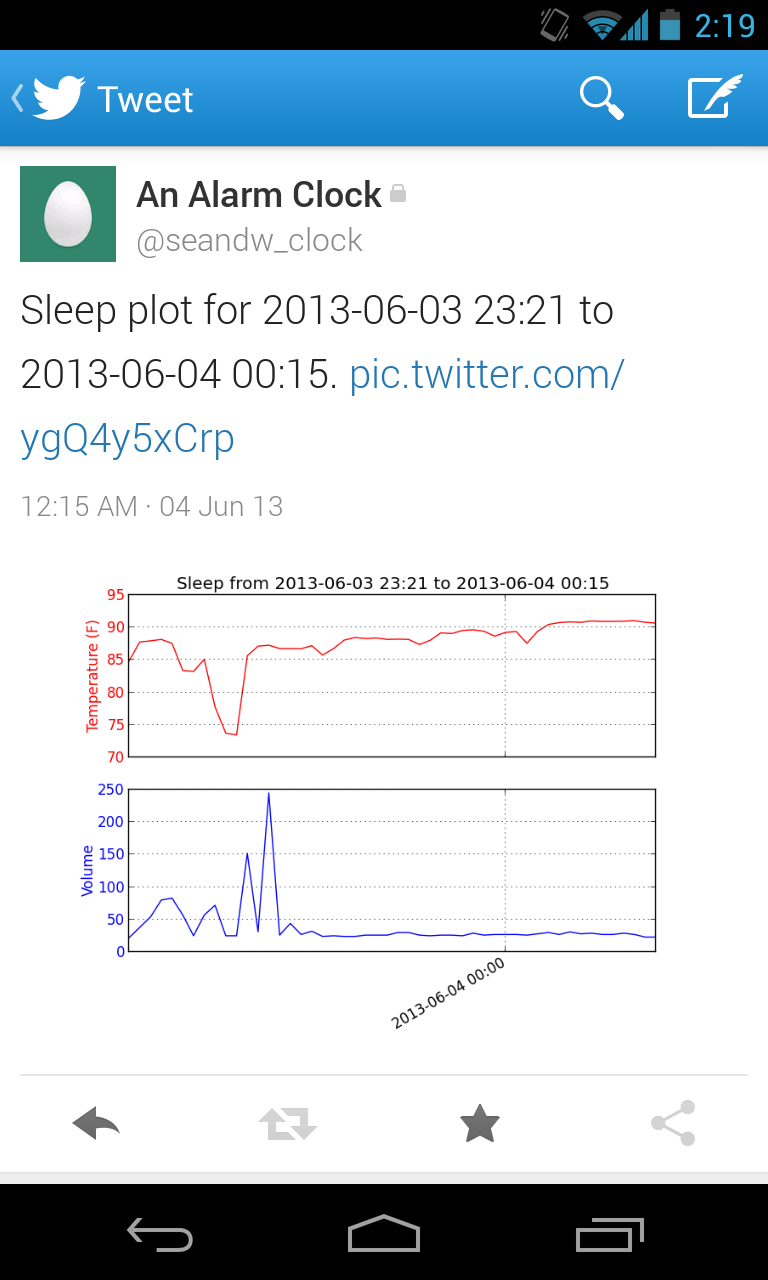
\includegraphics[width=0.5\textwidth]{twitmetrics}
  \caption{A tweet with a graph of statistics grathered during the
    sleep state.}
\end{figure}
